\documentclass{labReport}
\urlstyle{same}

\let\verbatim\undefined 
\let\verbatimend\undefined 
\lstnewenvironment{verbatim}{\lstset{breaklines,basicstyle=\ttfamily}}{}
\usepackage{lipsum}

\title{Lab 3: Iterative Algorithms}
\author{Adam Haile, Aiden Miller, Leigh Goetsch}
\prof{Dr. Berisha}
\className{Algorithms \& Adv. Data Struct.}
\classCode{CSC 3310}
\semester{Fall 2024}
\submissionDate{10/26/2024}
\labWeek{6}
\laboratoryDate{10/11/2024}

\begin{document}
\maketitle

\section*{Learning Outcomes}
\begin{itemize}
    \item Design an algorithm for a given computational problem statement
    \item Justify the correctness of an algorithm
    \item Perform asymptotic complexity analysis of the run time of an algorithm
    \item Generate test cases for an algorithm
    \item Correctly implement an algorithm from pseudocode
    \item Design and execute benchmarks for an algorithm
\end{itemize}

% if you want a TOC:
% \tableofcontents

\newpage
% if you want to use multicols:
\begin{multicols*}{2}
\raggedcolumns

For this lab we selected \\\textit{\textbf{Problem 1: Determine if a Point is Located Inside a Polygon}}.\\ The challenge is to determine whether a point lies inside or outside a polygon. The inputs are:
\begin{itemize}
    \item A sequence $<p_1, p_2, ..., p_n>$ of $n \geq 3$ 2D points.  Each point is a pair of x and y coordinates.  The points correspond to the vertices of a simple (non-intersecting) polygon.  The polygon is connected by line segments between each adjacent pair of points, including a line segment from the last point to the first point.
    \item The x and y coordinates for a single point distinct from the vertex points.
\end{itemize}
The output is:
\begin{itemize}
    \item A Boolean value indicating whether the point is located inside the polygon.
\end{itemize}

\section{Decision Rule}
% A paragraph describing a “decision rule” that can be applied to solve to the computational problem. Provide at least 2 illustrations (test cases) that demonstrate how the rule is applied.

Draw a horizontal line originating from the point infinitely to the right. 
If the number of times the line intersects with the point is odd, the point is located inside the polygon.

\begin{figure}
     \centering
     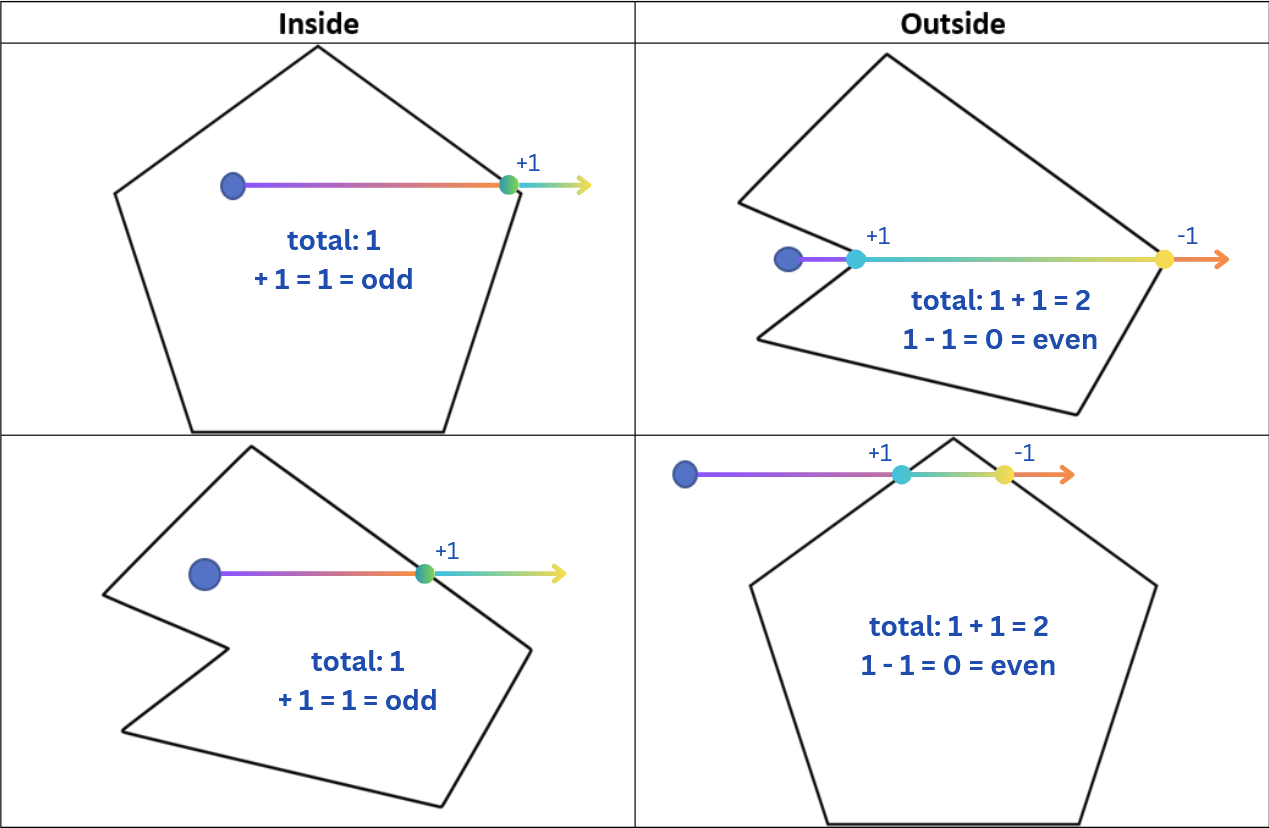
\includegraphics[width=1\linewidth]{images/decision_boundary.png}
\end{figure} 

\vspace{5em}

\section{Pseudocode}
% 2. High-level pseudocode for an algorithm that uses that rule to solve the computational problem for any input
\begin{verbatim}
inclusive = false
points = [list of polygon points]
distinct_point = (x, y)

vectors = drawVectors(points)
right_line = rightVector(distinct_point)

wn = 0
for vector in vectors:
    if counterclockwise_check(vector, right_line) or onsegment_check(vector, right_line, inclusive):
        wn += 1

return wn % 2 == 1
\end{verbatim}
\textbf{Explanation:}

\begin{itemize}
    \item For each vector, check if the line intersects. 
    \begin{itemize}
        \item If it intersects, increment. 
    \end{itemize}
    \item If the total is odd, return true.
\end{itemize}

\section{Algorithm Justification}
% 3. Provide an explanation and justification for why your algorithm is correct (1-3 paragraphs)
This algorithm can be proven using 

\section{Time Analysis}
% 4. Perform an analysis of the worst-case run time using asymptotic notation.

\section{Test Cases}
% 5. A table of your test cases, the answers you expect, and the answers returned by running your implementation of the algorithm.


\section{Benchmarking}
% 6. A table and graph from benchmarking your implementation on problem instances of different sizes. The benchmarks should support your theoretically derived run time.


\end{multicols*}

% add appendix
% 7. Attach all your source code and test cases in an appendix.



\end{document}
